\section{\label{sec4}Alignment of apparatus}
\subsection{Optical alignment}

An optical survey was performed for securing a good alignment of the
X-ray survey apparatus with respect to the calorimeter.  Following
this procedure X-ray coordintes from the motion controllers 
can be simply translated in to standard MEG coordinates.
The motion stages allow the X-ray to be moved in axial (Z) and
azimuthal ($\phi$) directions.  Using  an optical survey the axial
motion of the collimator is aligned to coincide with the MEG Z~axis.
Additionally, the rotational plane of the collimator is also aligned
to the vertical plane.  This procedure is performed by measuring the
exact coordinates (x,y,z) and the rotation plane vectors (rx,ry,rz) of
the X-ray at multiple reference axial locations.  Minor
deviatons from the expected positions are recorded and subsequently
used in the correction procedure (next section).  The precision of the
alignment X-ray postion at the calorimeter is calculated to be 0.1~mm
(0.15~mrad) in Z ($\phi$).

\subsection{Degrees of freedom of the X-ray beam}
\label{sec:corrections}
    Small displacements in the linear stage during its motion
    introduces rotations in the X-ray beam. The changes in
    the X-ray position are monitored using a laser attached to the
    linear stage projected at a quadrant photodiode, and a bubble
    level. The laser system detects difference in intensity of the
    laser in horizontal and vertical directions which are translated
    into angular deviations about X and Y axes. Figure \ref{fig:dxdy}
    shows axial position dependent relative intensities in horizontal
    ($\frac{\mathrm{left-right}}{\mathrm{total}}$, blue) and vertical
    ($\frac{\mathrm{down-up}}{\mathrm{total}}$, red) directions and the
    corresponding angular deviations $<\pm$0.8~mrad.
    \begin{figure}[]
      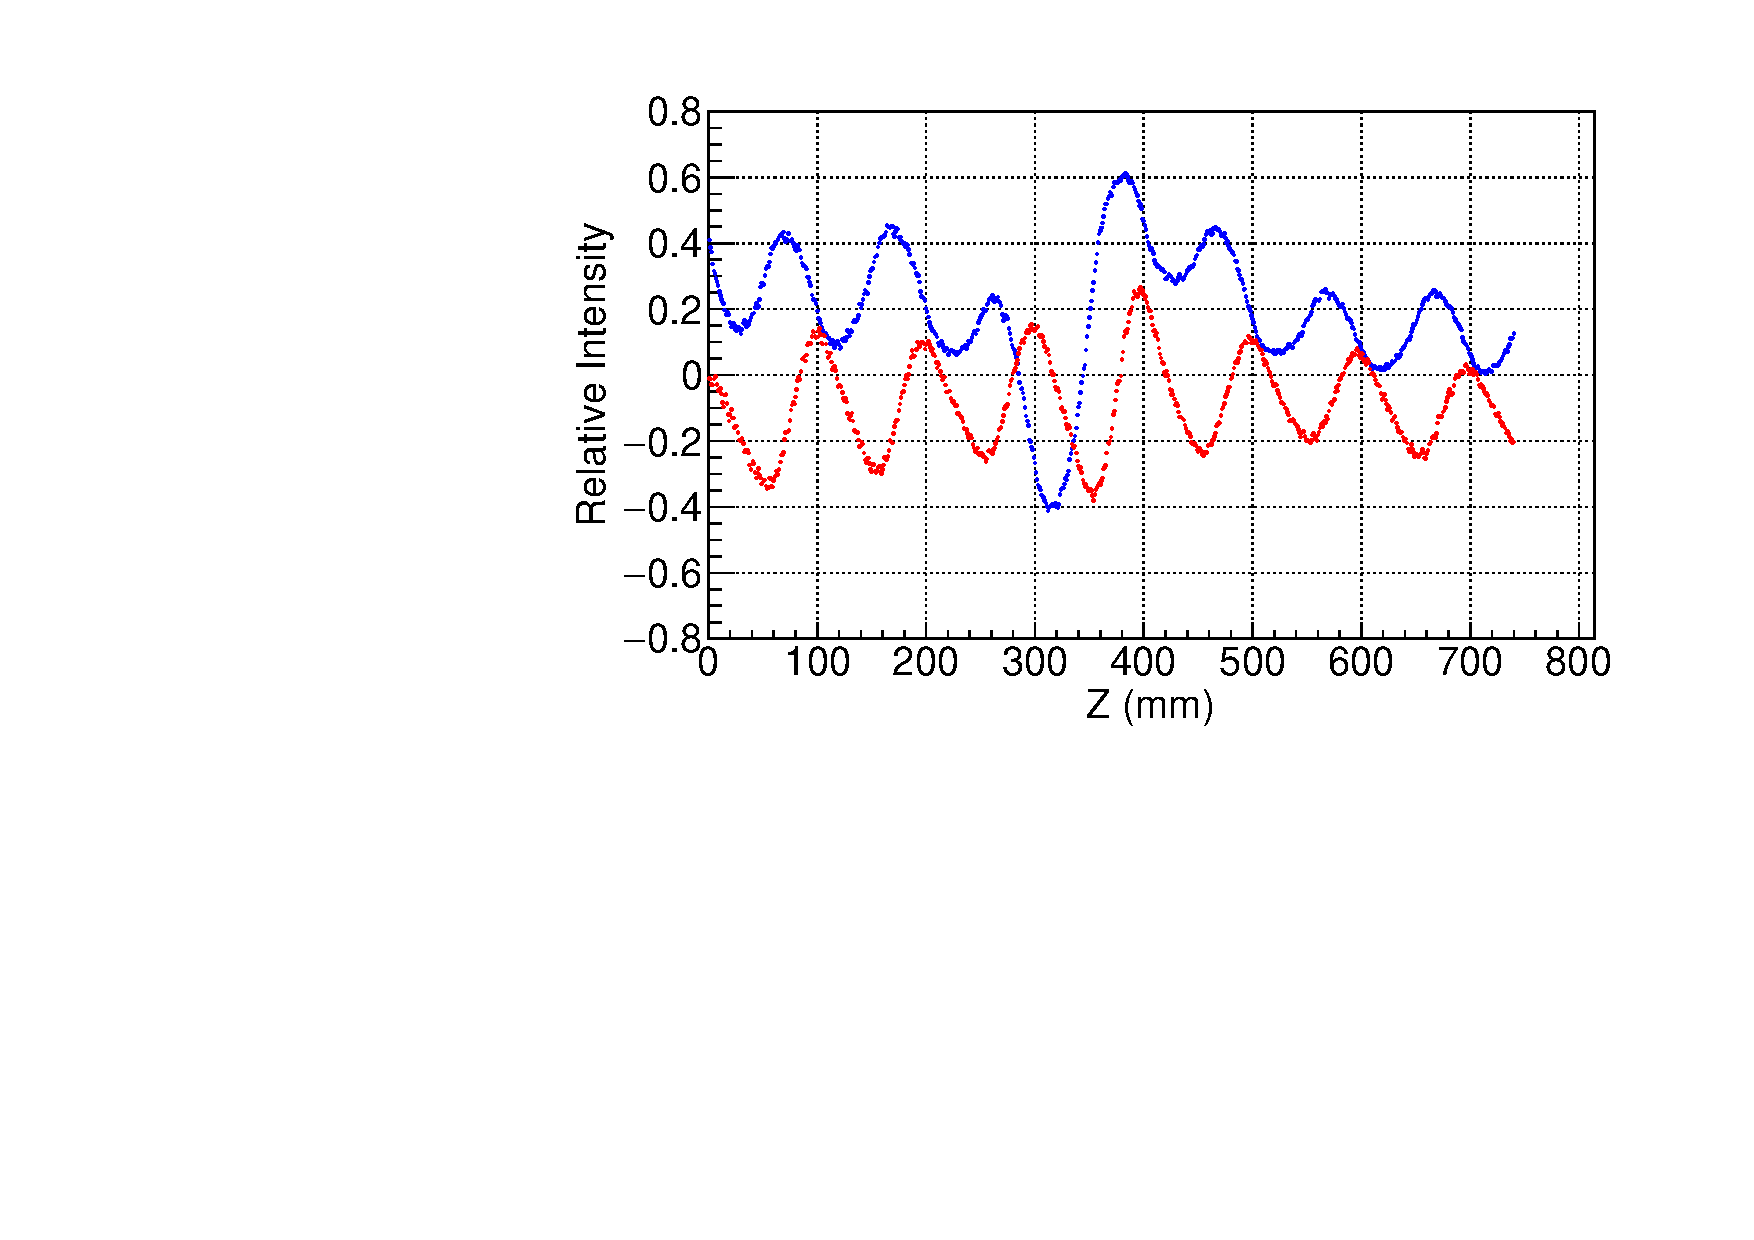
\includegraphics[width=4cm]{plots/rel_intensity}
      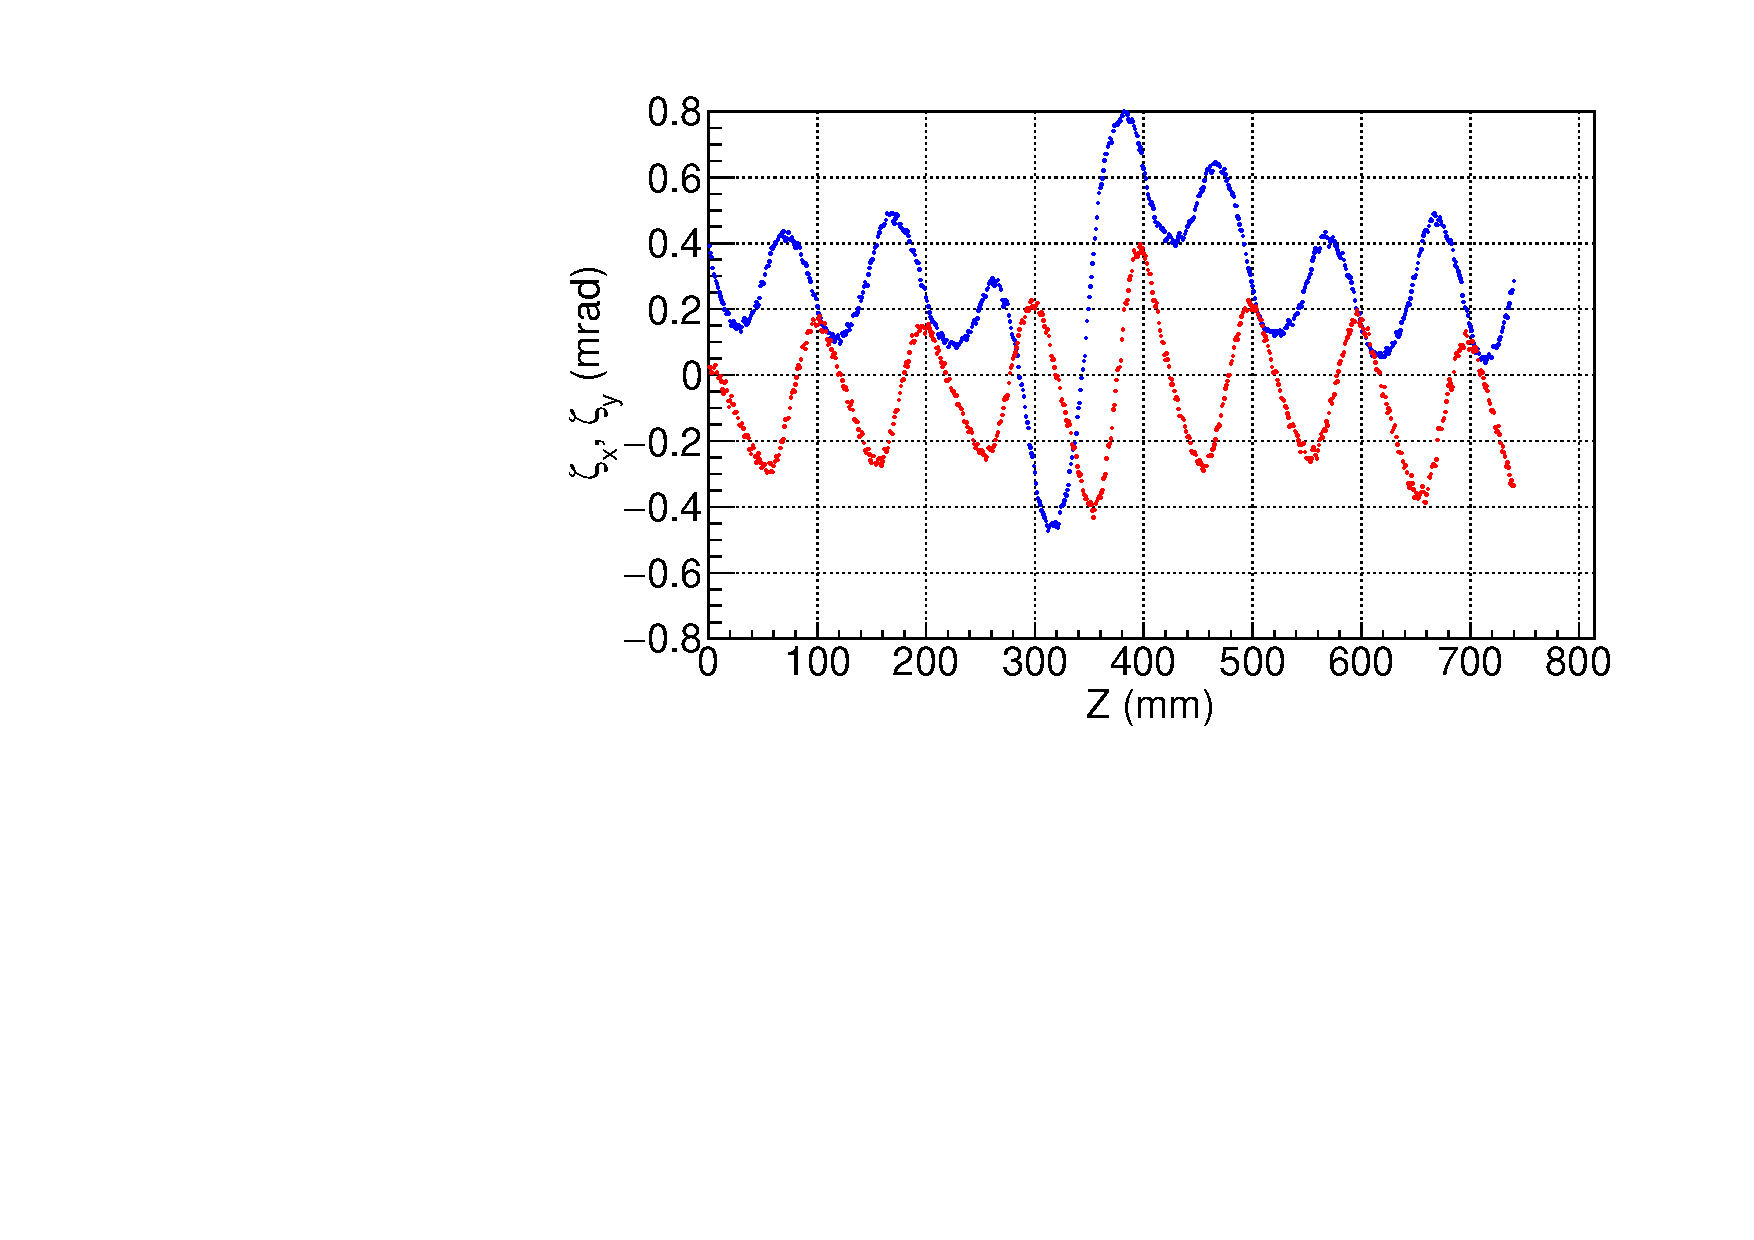
\includegraphics[width=4cm]{plots/angle_dx_dy}
      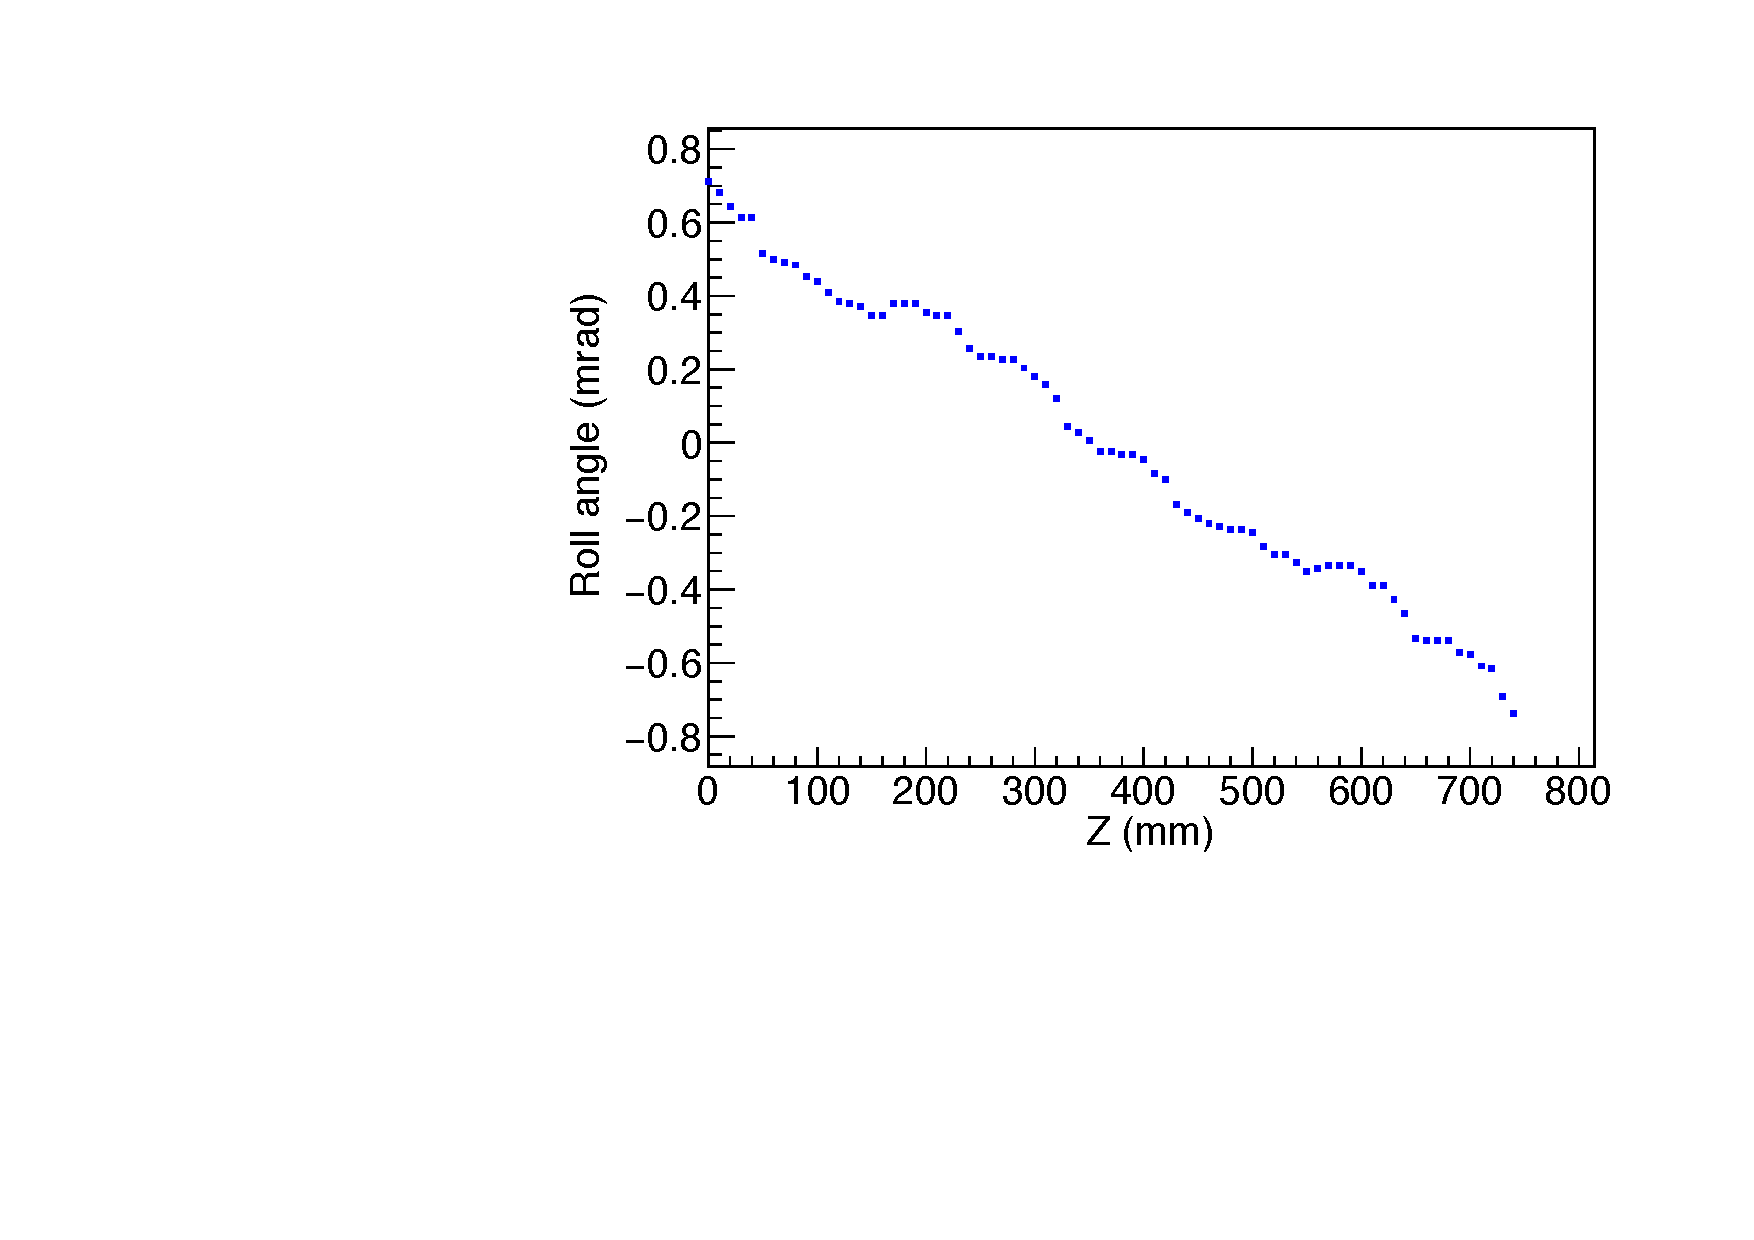
\includegraphics[width=4cm]{plots/BubbleLevel_June042017}
      \caption{Relative intensities in horizontal and vertical planes
      recorded by the laser monitoring system (left) and the calculated angular
      rotation (right).}

      \label{fig:dxdy}
    \end{figure}  
    The X-ray is projected in an orthogonal direction to the axis of the
    magnet. Working in the MEG coordinate system, the rotations of the
    X-ray about X and Y axes lead to a displacement in the Z coordinate of
    the X-ray at the calorimeter. For given angular rotations,
    $\zeta_x,\zeta_y$ about X and Y axes respectively, the correction in Z
    ($\Delta$Z) is proportional to the distance to the calorimeter (R) and
    the azimuthal angle ($\phi$) calculated as following

    \begin{align}
      \Delta Z(Z,\phi)_x &= -\zeta_x(Z)\,R\,cos(\phi)     \\
      \Delta Z(Z,\phi)_y &= \quad \zeta_y(Z)\,R\,sin(\phi) \\
      \Delta Z(Z,\phi)\  &= \quad \Delta Z_x + \Delta Z_y
    \end{align}

  A bubble level is used to detect the rotation of the X-ray
  collimator about Z~axis.  The position of the bubble is recorded
  with a 2~MP camera connected to Raspberry Pi device over the entire
  range of the linear stage.  A photograph is taken every 10~mm and
  the position of the bubble is interpolated at all intermediate
  locations. The photographs provide raw data which is converted into
  relative position of the bubble using pixel tracking
  software\cite{imagej} and calibrated to absolute rotation angle
  using the optical survey data(Figure~\ref{fig:bubblelevel}).  A
  correction is equal to the rotation angle about Z~axis, is added to
  the nominal $\phi$ value. Nominally, the X-ray collimator is fixed
  to the rotation stage    such that the centers of collimator and the
  rotational motion     coincide. However, optical surveys performed
  in the running period     show slight misalignment between the two
  in the vertical plane     ($\sim$100$\micron$).  This induces a
  $\phi$ dependent shift in the     $\phi$ coordinate of the X-ray;
  the effect on the Z coordinate is     found to be negligible. The
  correction to $\phi$ coordinates are calculated analtically
  considering the change in nominal and     displaced X-ray vectors at
  the calorimeter. Given the angular     rotation $\zeta_z$ about
  Z-axis, and the angular offset $d\phi_{coll}$     due to displaced
  collimator center, the $\phi$ correction      ($\Delta\phi$) is
  calculated as 

  \begin{align} 
  \Delta \phi (Z,\phi) = \zeta_z(Z)+d\phi_{coll}(Z,\phi) 
  \end{align}

  %%Z axis in plots must be converted to MEG coordinates, axis labels.
    \begin{figure}[]
        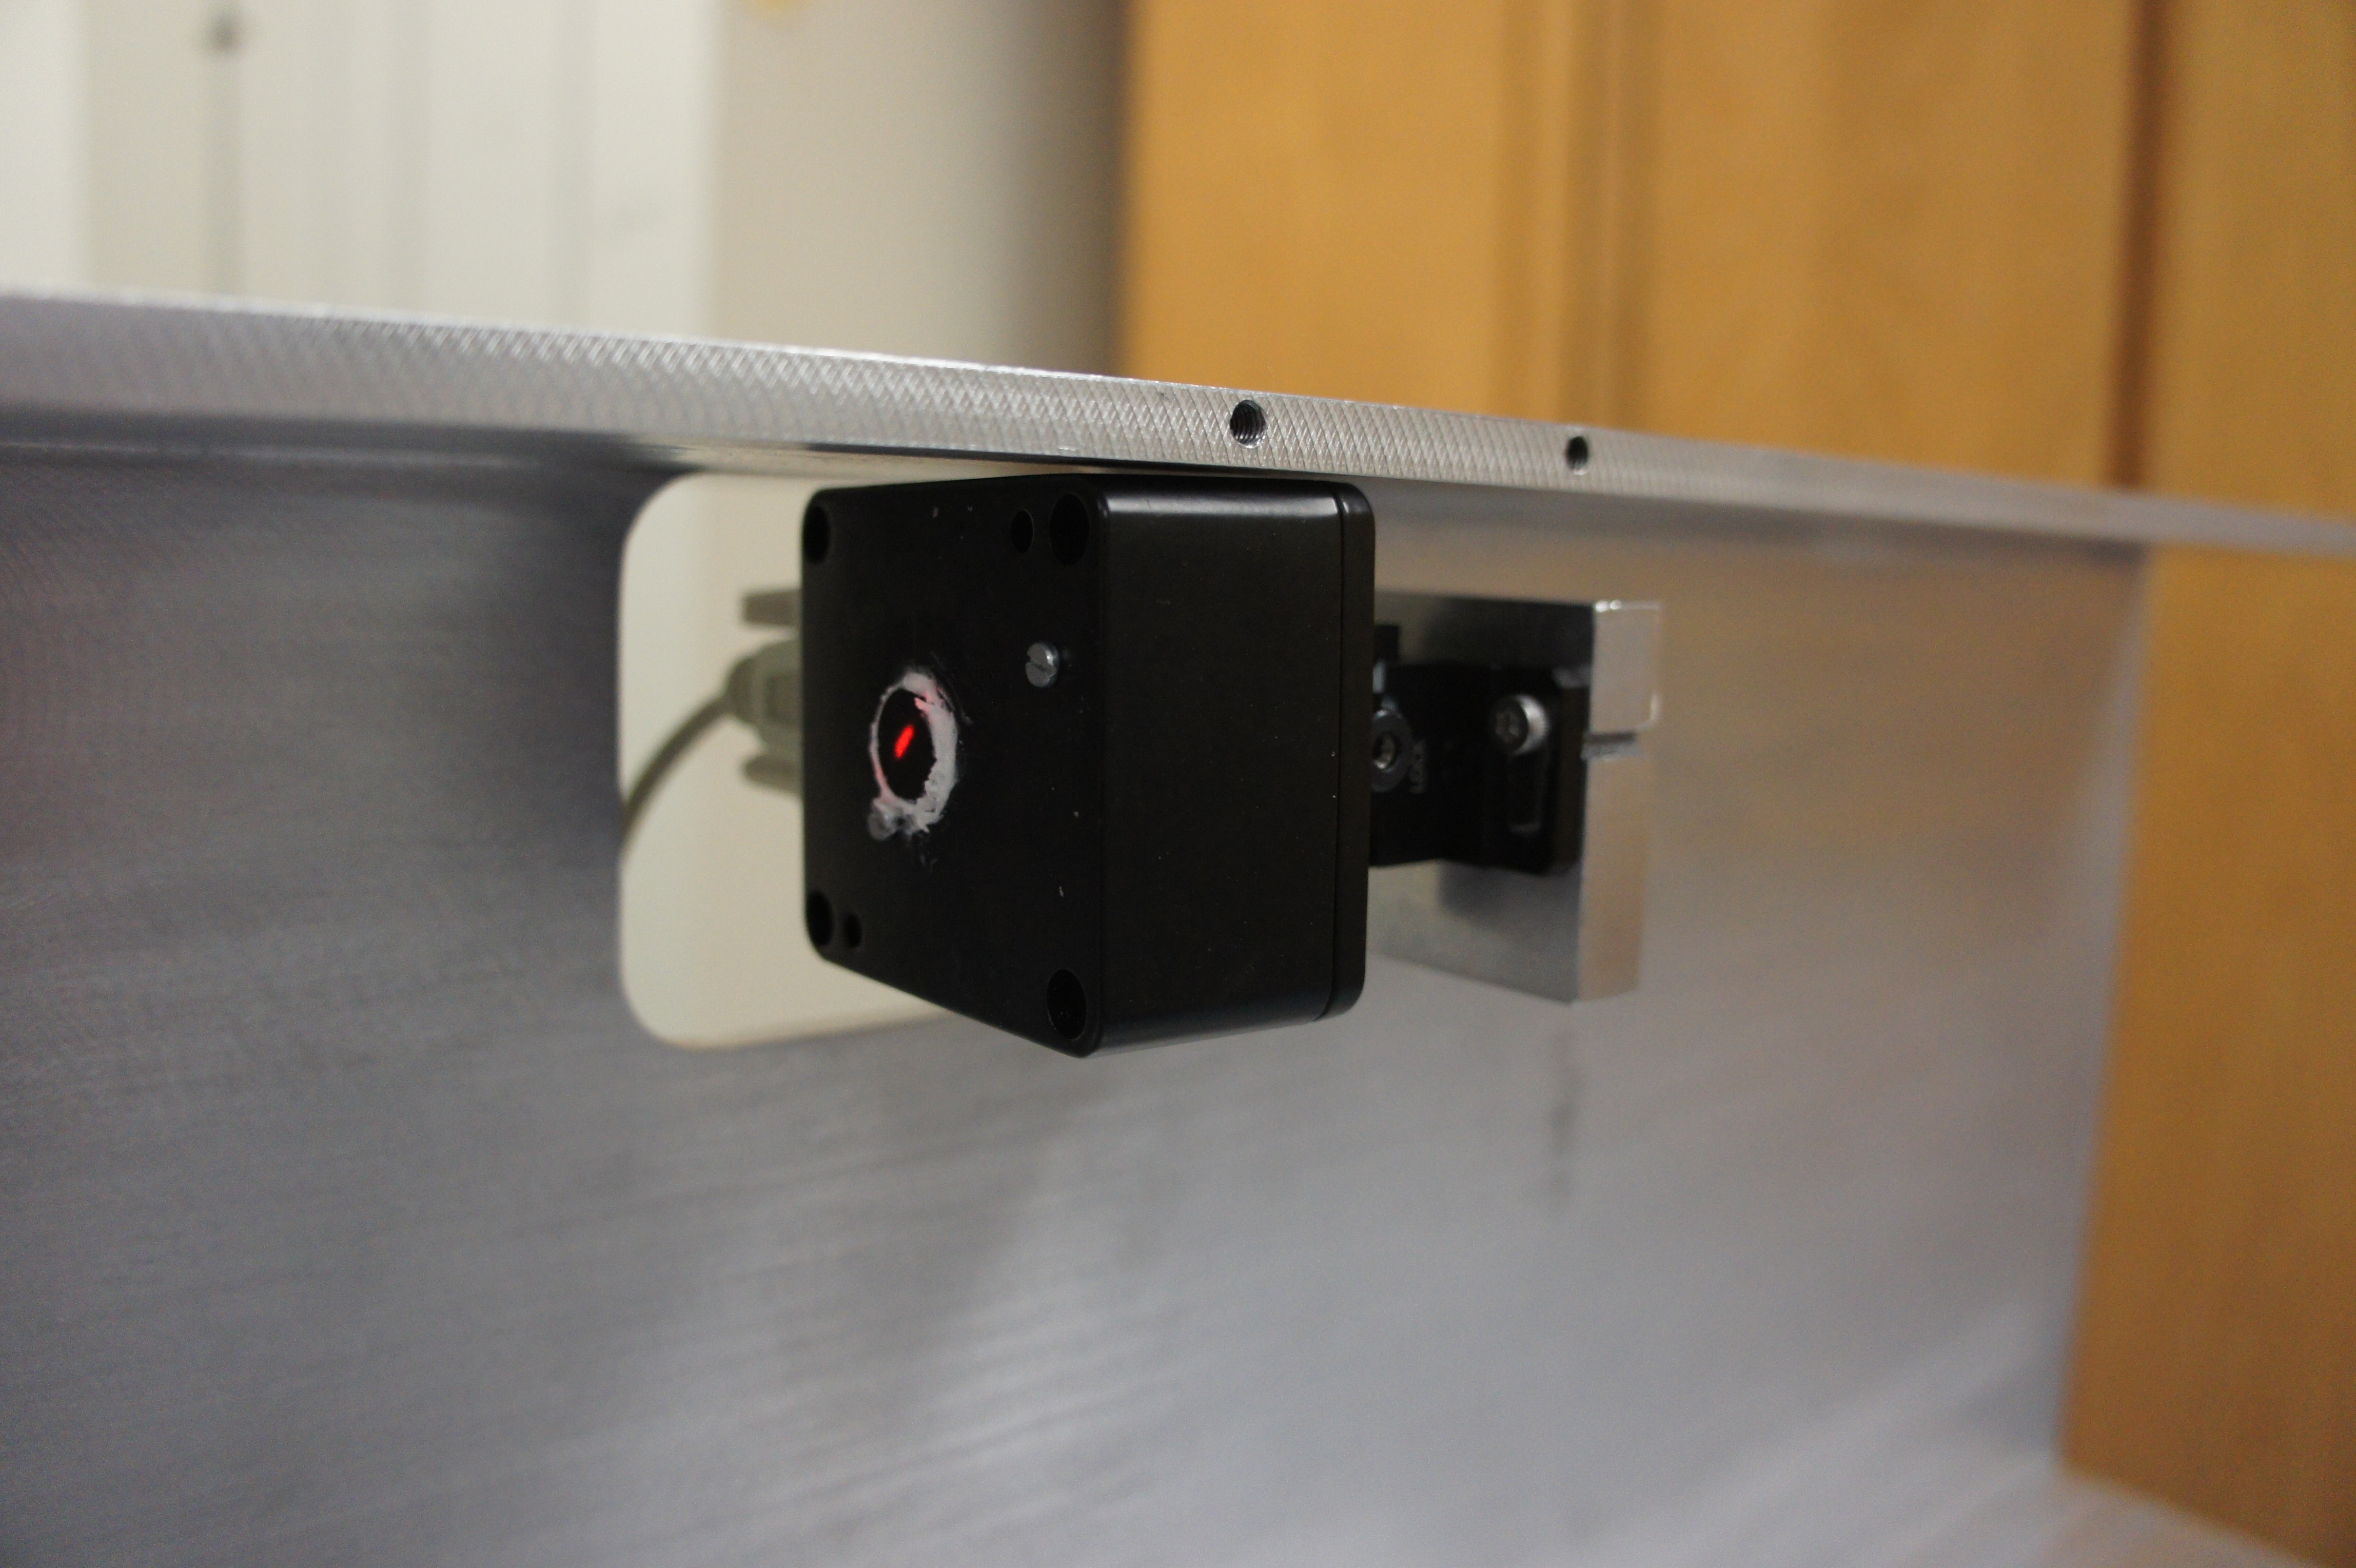
\includegraphics[width=4cm]{plots/qpd.jpg}
        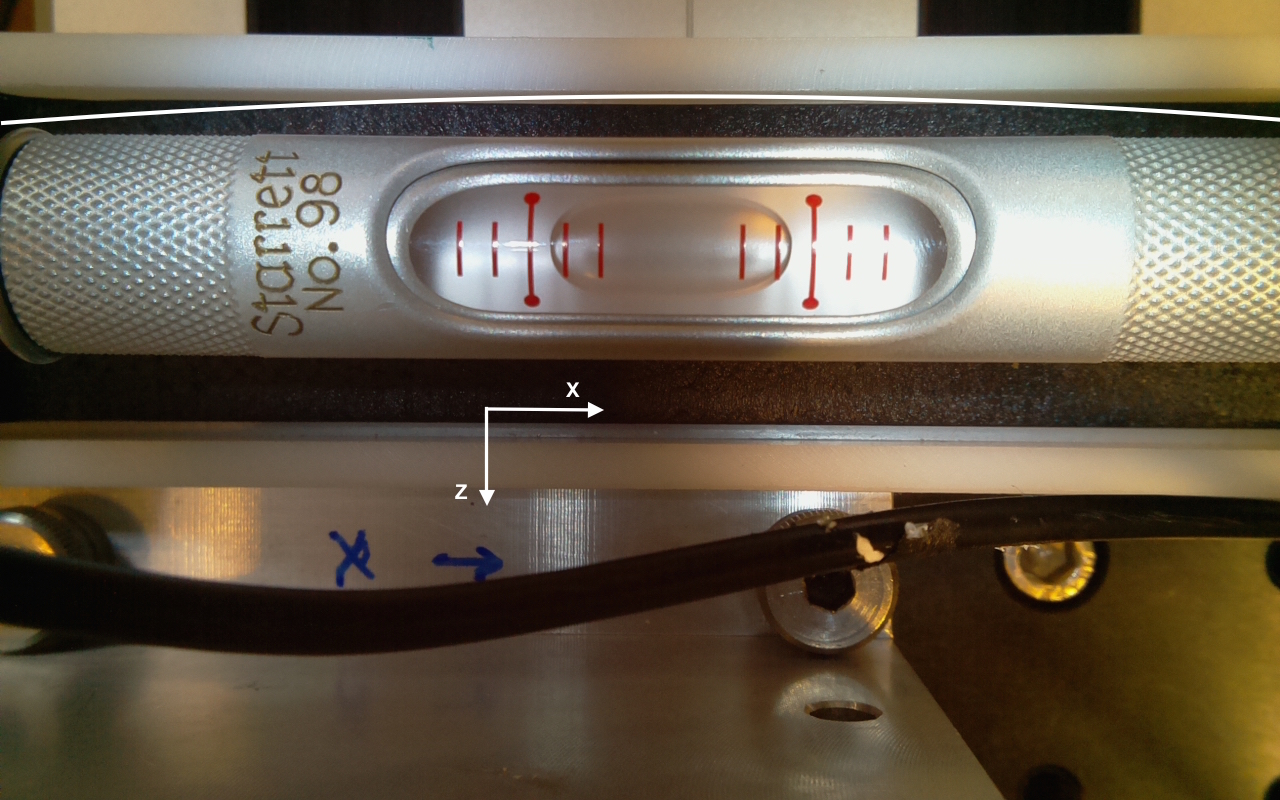
\includegraphics[width=4cm]{plots/whitetray.jpg}
      \caption{The quadrant photodiode (left) and the bubble level
                (right) for measuring rotations about the primary
                axes.}
      \label{fig:bubblelevel}
    \end{figure}  


      %%\subsection{Corrections to the beam position}
      %%
      %%%Relative angles measured by the bubble level are normalized to the
      %%%reference measurement made by the optical survey at the axial center
      %%%Z = 0 mm.
      %%Secondly, the rotation of the X-ray collimator about Z~axis 
      %%to the $\phi$ coordinate of the X-ray equal to the angle  of 
      %%rotation. 
      %%
      %%The $\phi$ correction ($\Delta \phi$) The rotation of the X-ray about
      %%Z-axis introduces a correction to the phi coordinate of the X-ray
      %%equal to the rotation angle.  The rotation about Z axis displaces the
      %%X-ray $\phi$ equal to the angle of rotation. Hence, angular
      %%measurement from the bubble level, calculated in the right-handed
      %%reference frame, is added to the nominal $\phi$. 
      %%
      %%Another correction to the X-ray $\phi$ is required due to radial offset between the center
      %%of rotation and the Another correction to the $\phi$ coordinate is required due based on
      %%the 
      %%The $\phi$ correction is given by the measured Z rotation and the phi offset 



      %A radial offset between the
      %center of rotation and the collimator requires a $\phi$ dependent
      %correction, maximally calculated to 0.38~mrad.


      %%\subsection{Uncertainties}
      %%\label{sec:corruncertainties}
      %%Variation in the relative intensities of the laser leads to
      %%uncertainty on the angular rotations about X and Y axes. The
      %%uncertainty on the Z correction is calculated as maximum
      %%deviation allowed by the variation of the rotation angles in their
      %%uncertainty ranges. 
      %%
      %%The Z correction varies as a function of Z and
      %%$\phi$ between $\pm$0.6~mm with an average uncertainty of 0.03 mm
      %%(10\%).  The uncertainty in the rotation angle about Z axis ($\zeta_z$) is
      %%determined as the change in the angle calculated from two consecutive
      %%runs. The $\phi$ correction due to a rotation about Z axis ranges
      %%from -0.3 to 0.3 mrad and average uncertainty 0.12 mrad (40\%).
      %%Figure~\ref{fig:unc} shows the correction to the nominal coordinates
      %%of X-ray beam with uncertainties.
      %%
      %%
      %%\begin{figure}[]
      %%  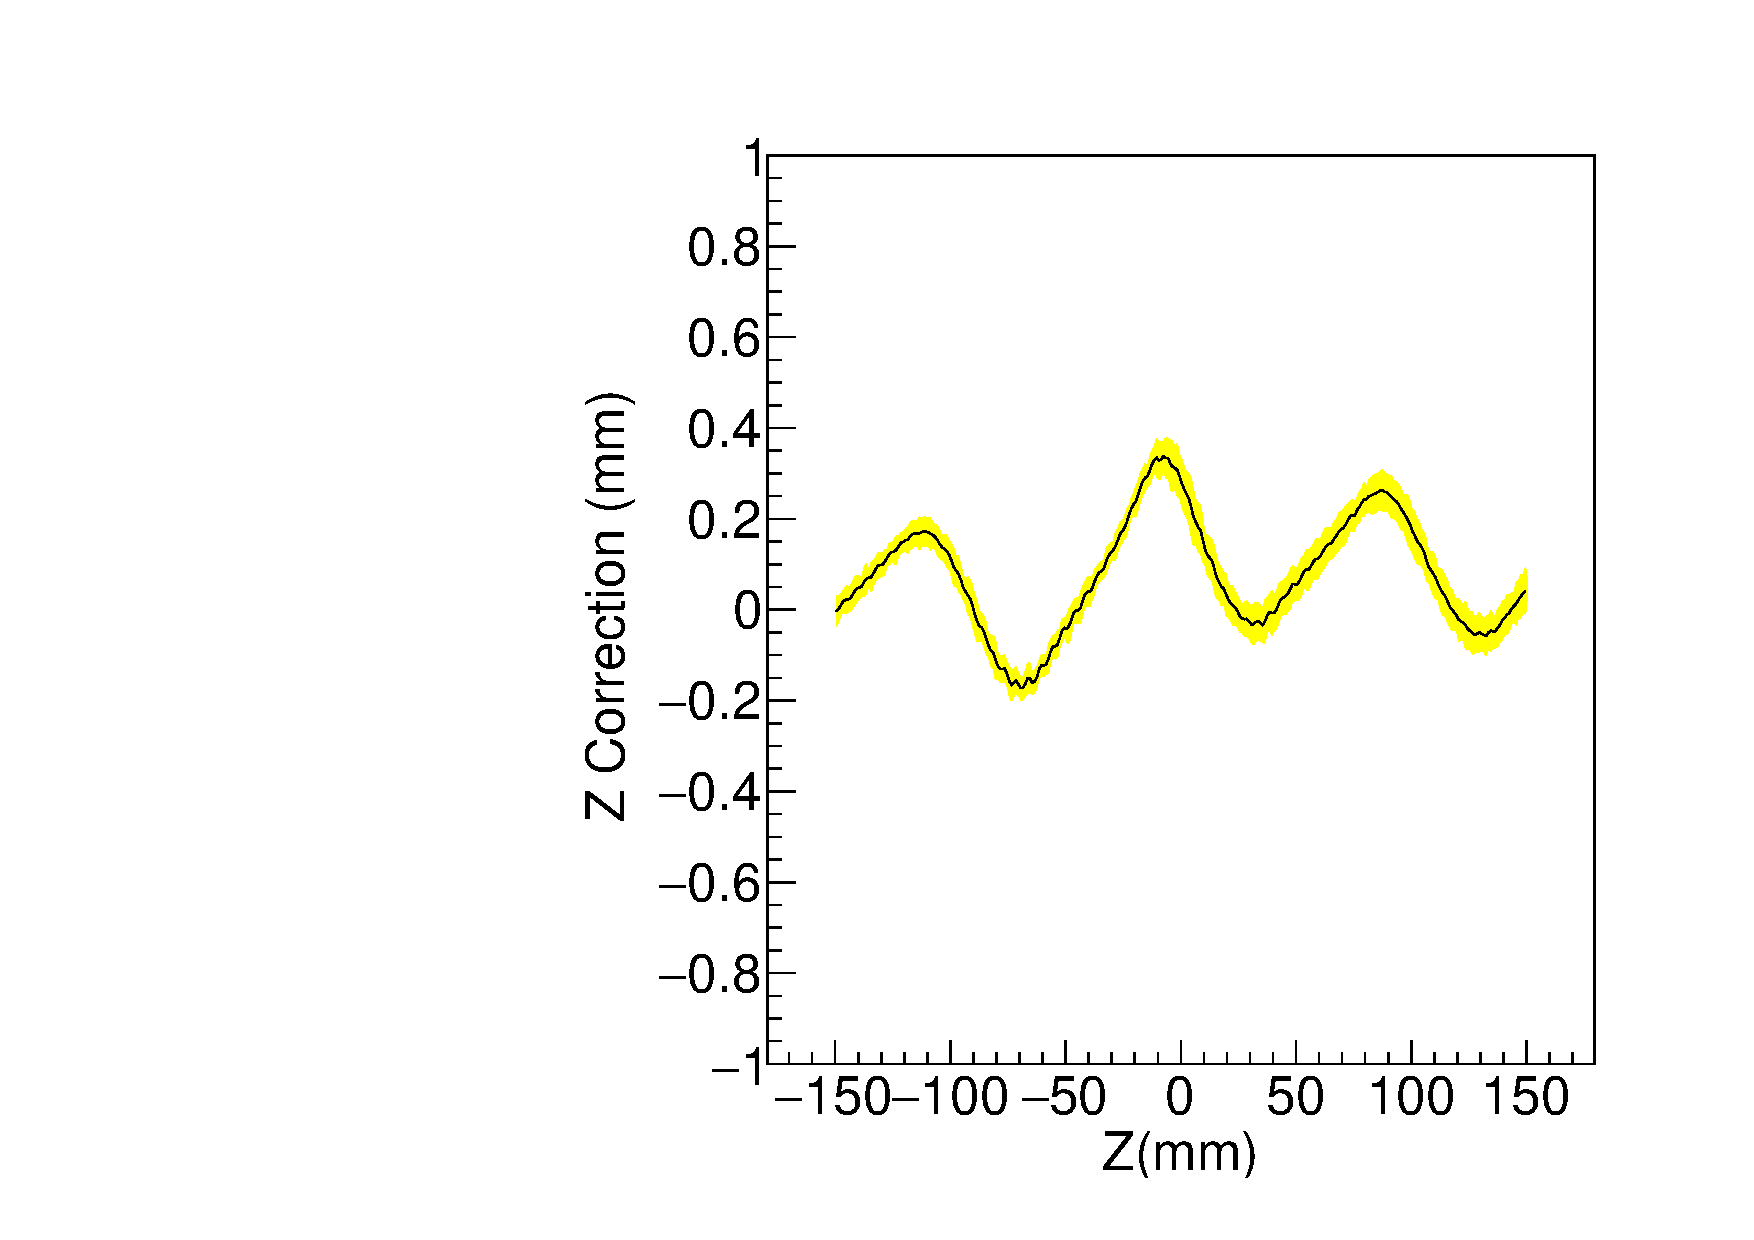
\includegraphics[width=7cm]{plots/cerr1}
      %%  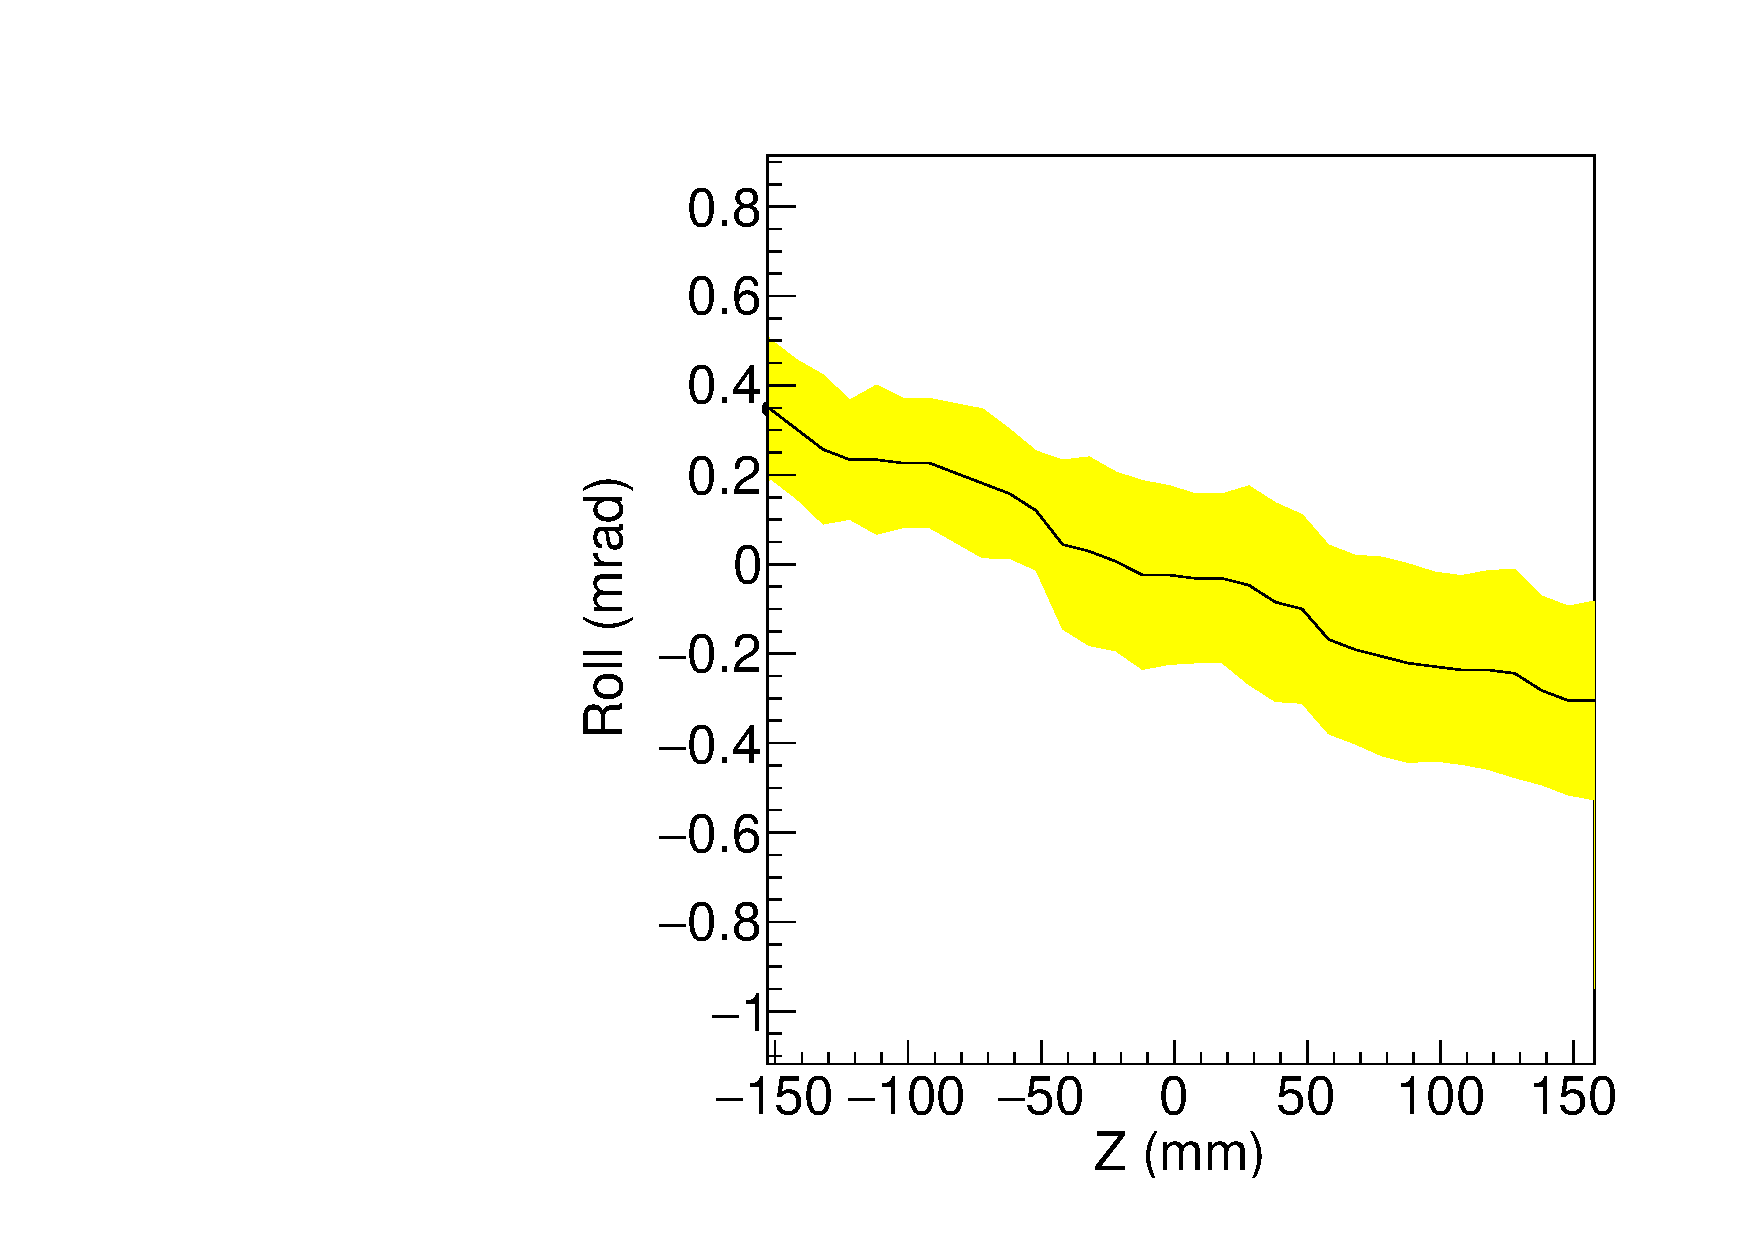
\includegraphics[width=7cm]{plots/rollUnc1}
      %%  \caption{Correction applied to X-ray coordinates Z and $\phi$ with
      %%  uncertainties.}
      %%  \label{fig:unc}
      %%\end{figure}  

